\chapter{Example Simulation Model}
\label{chapter:example-simulation-model}

\todo[inline]{ fix this
In this chapter, we present an example simulation model of Cavium OCTEON II CN6880 network processing unit~\cite{cavium:2010:fundamentals}.

First, we will introduce the Cavium OCTEON II CN6880 unit, and then describe the measurement setup required to obtain reference values for the simulation model. Two different measurements will be done, one to measure the communication latencies, and another to measure the memory latencies and throughput. Then, we will present the actual simulation model, including the model components and entities. The gathered reference values are plugged in to the model and the relevant details are discussed. Finally, we describe the implementation of the SSO unit using the PSE plugin interface.
}

\section{Characteristic Measurements}
\label{sec:characteristic-measurements}

For the model to represent the packet latencies and throughput with enough accuracy, the model needs to be filled with apposite entity parameters. Some of the model parameters are simple enough to be obtained directly from~\cite{cavium:2010:fundamentals}, while others are either unavailable, or are presented in an unusable form to be used in the simulation model. The missing communication and memory related parameters are obtained by conducting measurements on the real CN6880 hardware. These are discussed in the following sections, respectively.

% We believe that, by determining the latecies of input phase and output phase, the behaviour of memory, and modeling the packet scheduler with enough accuracy, the sought applications' effects to the packet latencies and throughput come up with enough accuracy.

% For our approach to be valid, i.e. the abstraction of the communication latencies to be precise enough, we have to assume the fastpath is not the bottleneck in the processing phase. This assumption is reasonable because ...

% \fixme{
%   TODO:
%   \begin{itemize}
%   \item because the fastpath hardware is optimized for this task
%   \item find reference
%   \item maybe justify the stuff with some kind of rough back-of-the-envelope calculation?
%   \end{itemize}
% }

\subsection{Communication Latencies}
\label{sec:communication-latencies}

By communication latencies, we refer to the time in the input and output phase of the packet processing, between physical receive/transmit ports and the actual core processing, as described in the Section~\ref{sec:cavium-octeon}. We will include the times spent in the SSO unit for both of these metrics, as due to our resource constraints, we were unable to do the measurements with the required detail to break down these delays. Also, for our modeling purposes, it is accurate enough to assume that the input and output phases consume equal amount of processing time.

The input and output phase latencies are measured by generating traffic from external machine, and passing it through two CN6880 units back to the generator itself. The measurements were done at two independent points in the processing path, to validate the accuracy of the measurements.

\begin{figure}[]
  \begin{center}
    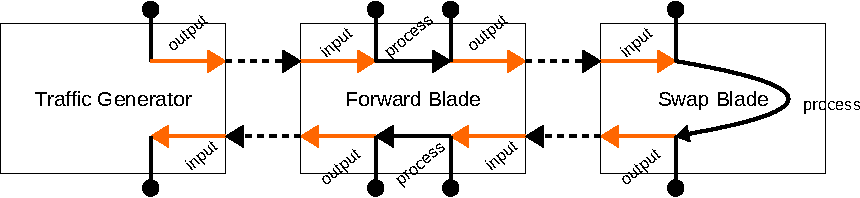
\includegraphics[width=\textwidth]{images/comm-measurement-setup.pdf}
    \caption{The setup used to measure the communication latencies. The communication between the nodes, packet processing on the main cores, and the input and output processing, are marked with the dashed arrows, solid black arrows, and orange arrows respectively. The probes present the points of measurement.}
    \label{fig:comm-setup}
  \end{center}
\end{figure}

In figure~\ref{fig:comm-setup}, the rectangles represent three different computing units (traffic generator, forward unit, and swap unit), and the probes present the points of time measurements. The traffic generator is a typical desktop computer running Ubuntu operating system, and the traffic was generated by Mausezahn~\cite{mausezahn}. Both of the Octeon CN6880 units are running Linux operating systems.

The packet is first generated at the packet generator and sent to the forward unit at time $t^{d}_{0}$. Forwarding unit receives the packet at time $t^{r}_{10}$, does the required processing and forwards the packet to the swap unit at time $t^{d}_{10}$. The swap unit receives the packet at time $t^{r}_{2}$, does the same processing as the forward unit (except with different destination address), and forwards the packet back to the forward unit at time $t^{d}_{2}$. Finally the forward unit receives the packet at time $t^{r}_{11}$ and forwards it to the traffic generator at time $t^{d}_{11}$, which marks it received at time $t^{r}_{0}$. The time $t_{f}$ spent in the input and output phase of one unit is then

\begin{equation}
  \label{eq:1}
  t_{f} \approx \frac{t^{r}_{11} - t^{d}_{10} - (t^{d}_{2} - t^{r}_{2})}{2}.
\end{equation}

We measured the times for packet sizes of 64B, 128B, 256B, 512B, 1024B, and 1500B, repeating the measurement for each packet 10000 times. Figures~\ref{fig:comm-latency-boxplot} and~\ref{fig:comm-latency-histograms} present the statistics of the resulting times $t_{f}$ for the different packet sizes.

\begin{figure}[]
  \begin{center}
    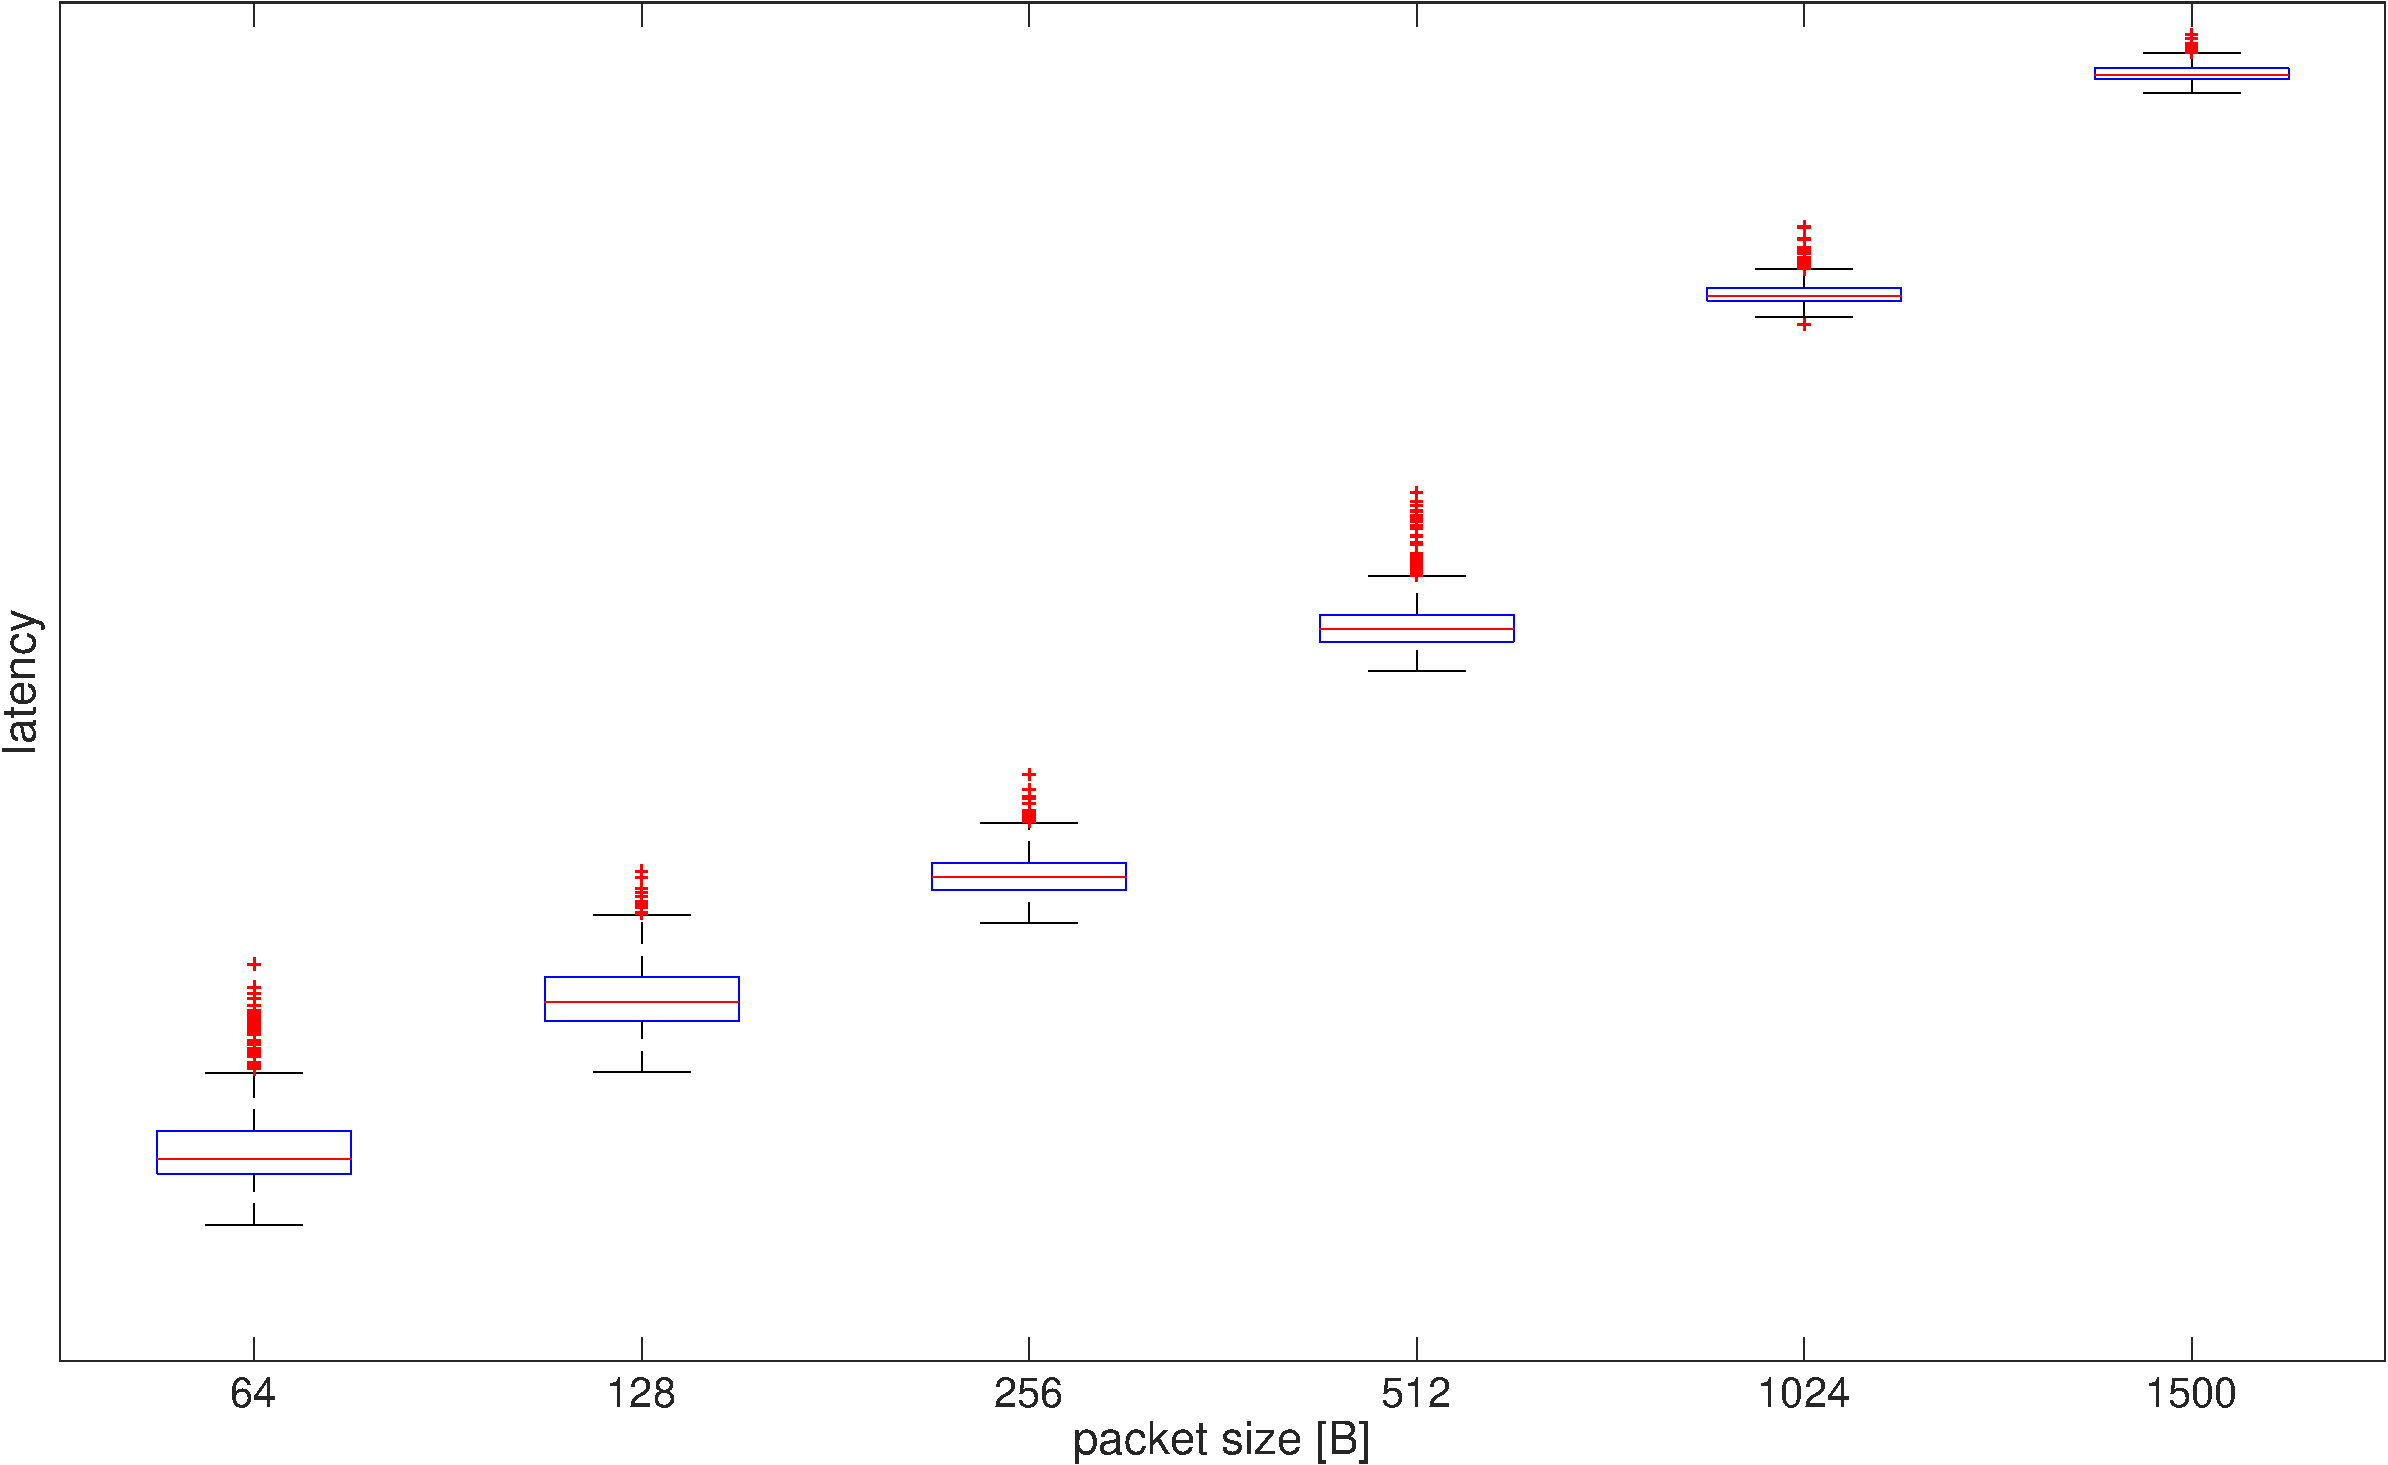
\includegraphics[width=\textwidth]{images/comm-latency-boxplot.pdf}
    \caption{Latency of the input and output phase of the CN6880 unit. On each box, the central mark is the median, the edges of the box are the 25th and 75th percentiles. 99.3\% of the points lie within the whiskers, and the most extreme points are presented as red crosses. Both of the axes are on logarithmic scale.}
    \label{fig:comm-latency-boxplot}
  \end{center}
\end{figure}

\begin{figure}[]
  \begin{center}
    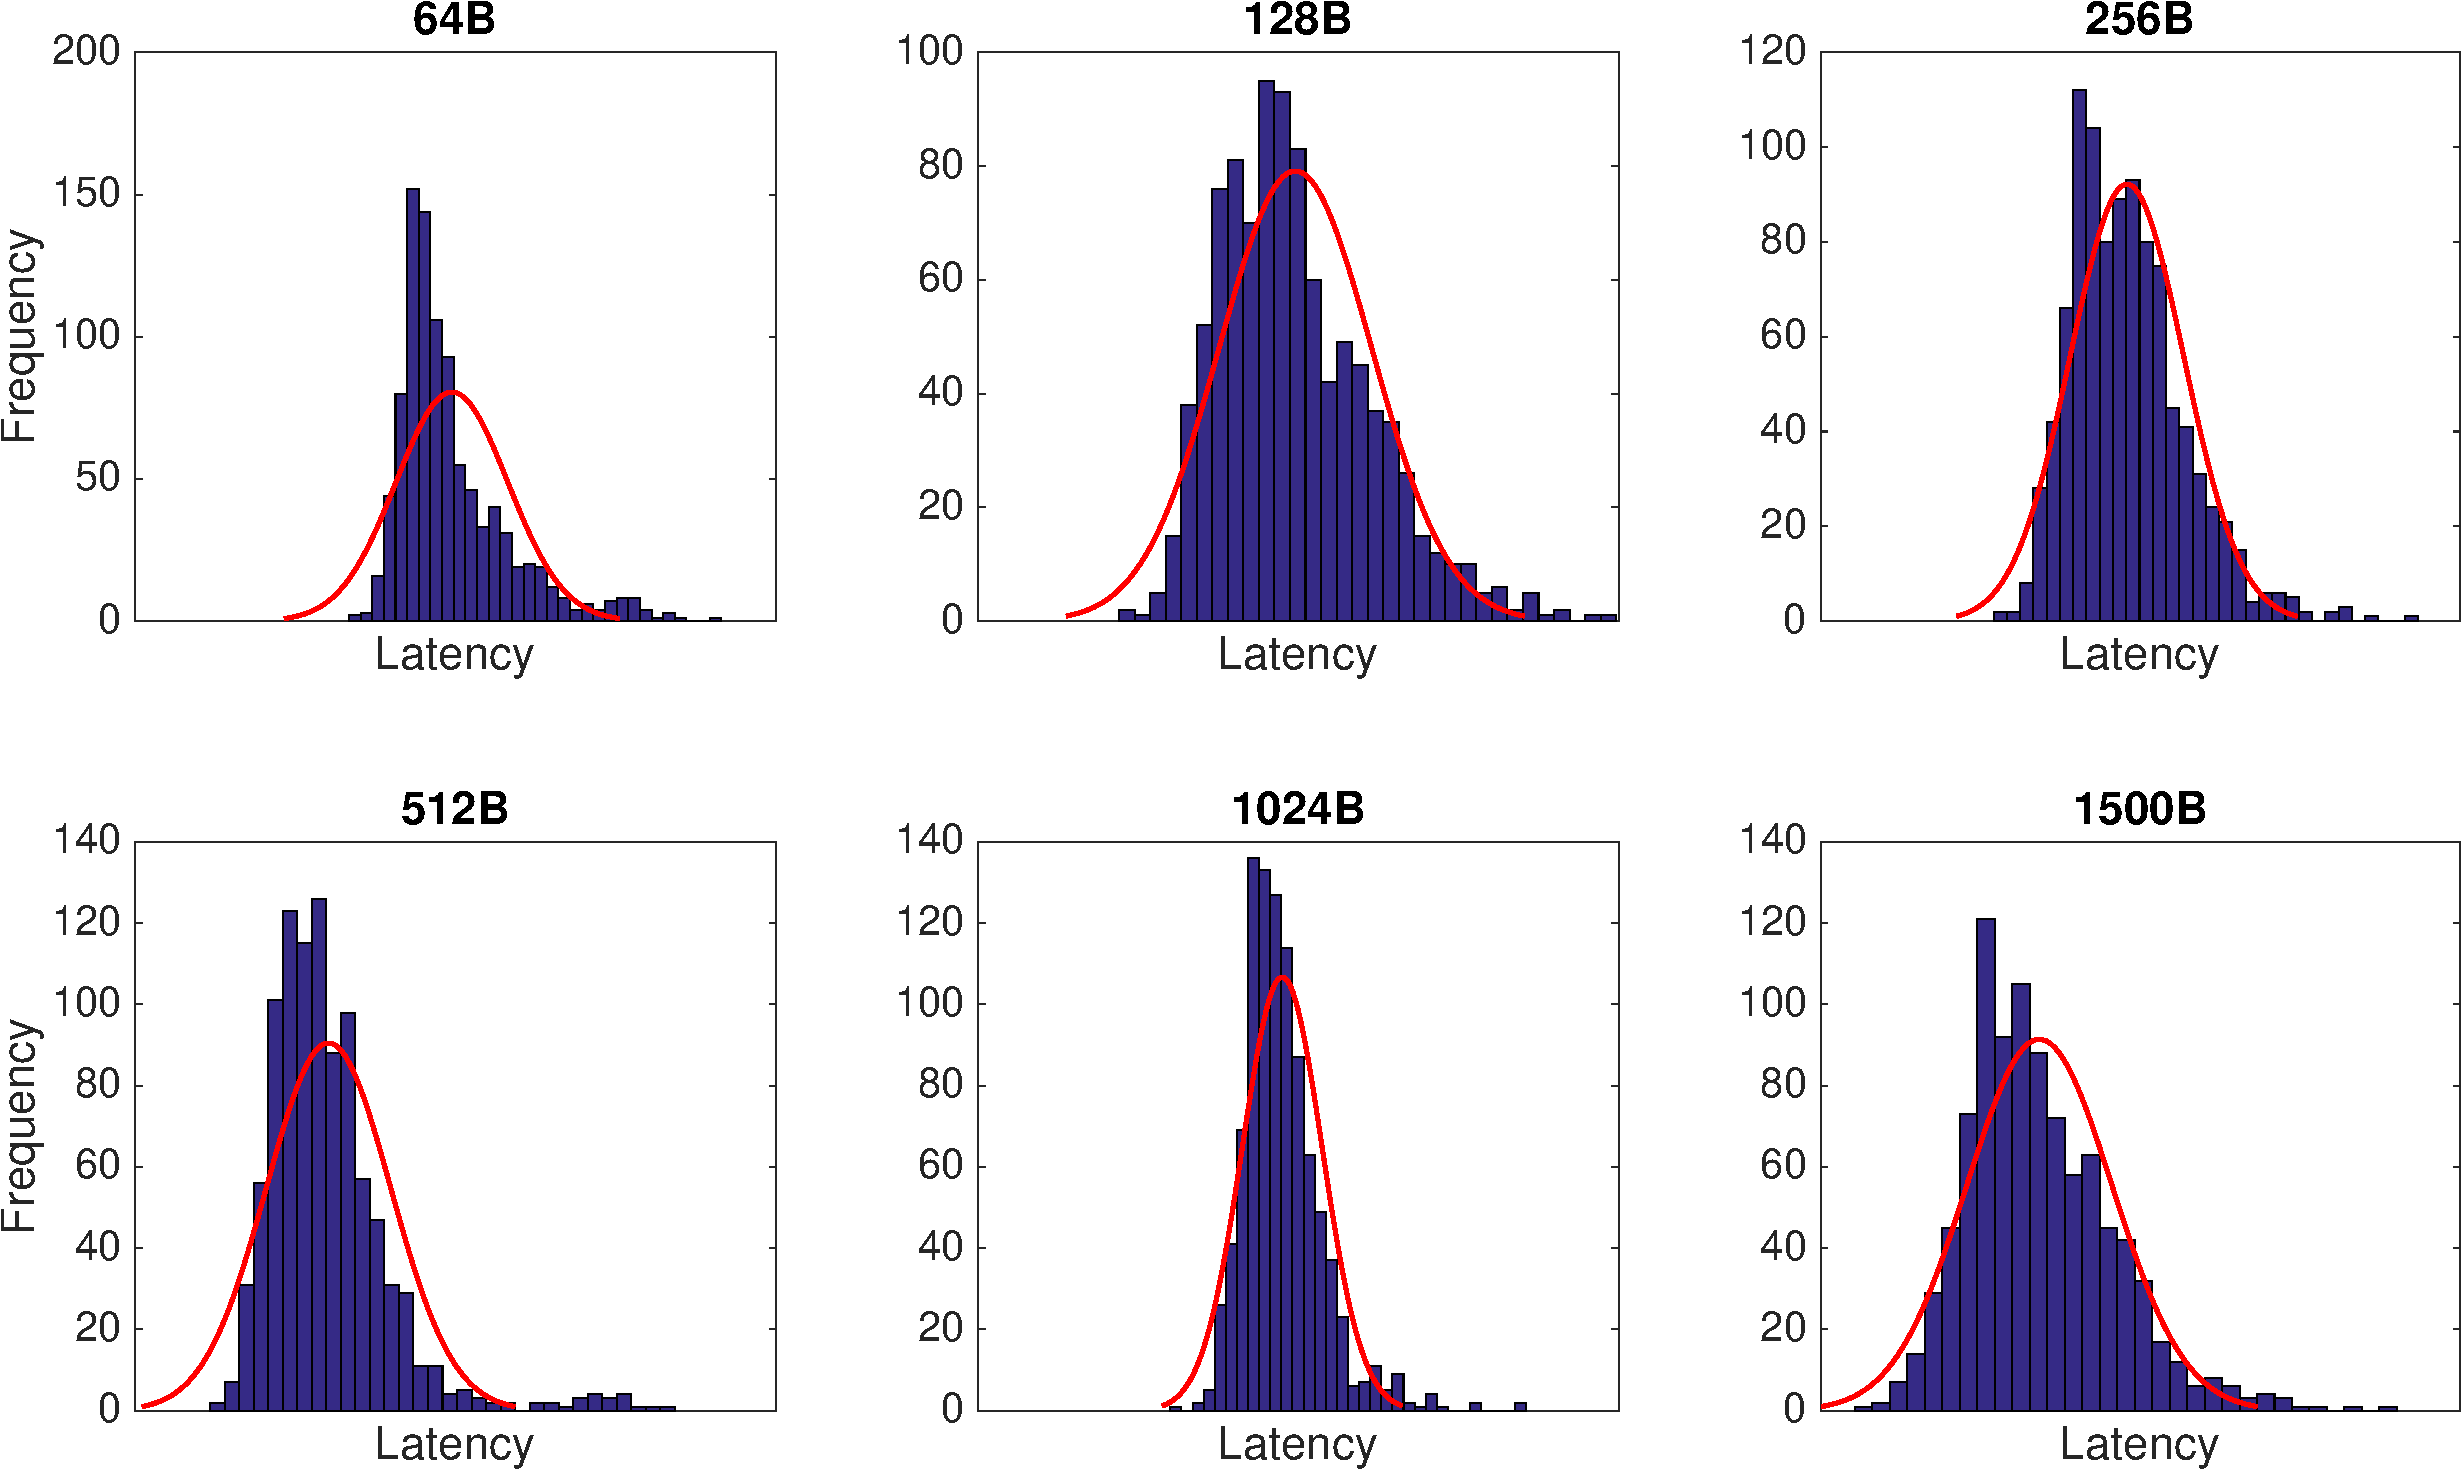
\includegraphics[width=\textwidth]{images/comm-latency-histograms.pdf}
    \caption{Latency frequency histograms for each packet size, along with a normal density function with parameters, estimated with maximum likelihood method from the data.}
    \label{fig:comm-latency-histograms}
  \end{center}
\end{figure}

As shown in the figure~\ref{fig:comm-latency-boxplot}, the time spent in the input and output phase of the unit is roughly linear regarding to the packet size. The variation of the data is relatively small on all packet sizes. The trend of the latency with respect to the packet size, corresponds to the trend of the values measured with at the external traffic-generator (which causes $3.1\mu s$ constant overhead regardless of the packet size). The corresponding plots for the external traffic-generator measurements are omitted for clarity.

As seen from both of the figures~\ref{fig:comm-latency-boxplot} and ~\ref{fig:comm-latency-histograms}, there exist points with unexpectly large deviation from the rest of the group. These deviations seem to be independent of the packet size, and thus we assume that they are caused by the scheduling unit (SSO). This behaviour is also statistically incorporated in the simulation model.

The only packet size dependent operations in the input and output phases are the memory transfers done for the actual packet data between the memory (L2/RAM) and PKI or PKO. All the other other operations are done based on the packet header, thus requiring constant amount of time regardless of the packet size.

Since We cannot make a distinction between the input and output phase, in the simulation model presented further, we will adjust the input/output phase amount so that they consume the PKI and PKO units for the amount that corresponds the constant term of equation~\ref{eq:1}. The variable (non-constant) term is caused by the memory copies in the input/output phases, and are proportional to the packet size.

The input and output delays used in the simulation model are estimated by fitting a linear model to the data, using least square estimate. The determination coefficient of the estimate $R^2 = 0.997$. The delay for the input and output phase are divided evenly, resulting in

\begin{equation}
  \label{eq:1}
  t_{in} = t_{out} = \frac{1}{2}(0.0018\frac{\mu s}{B} * packet\_size + 1.036\mu s).
\end{equation}

\subsection{Memory Characteristics}
\label{sec:memory-characteristics}

Memory delays were measured using Multi-core Processor Architecture and Communication (MPAC) benchmarking library~\cite{Jamal:2009:MPAC}. Both, latency and throughput, were measured using different dataset sizes and number of threads. Each of the tests were run on 200,000 repetitions.

\begin{figure}[]
  \begin{center}
    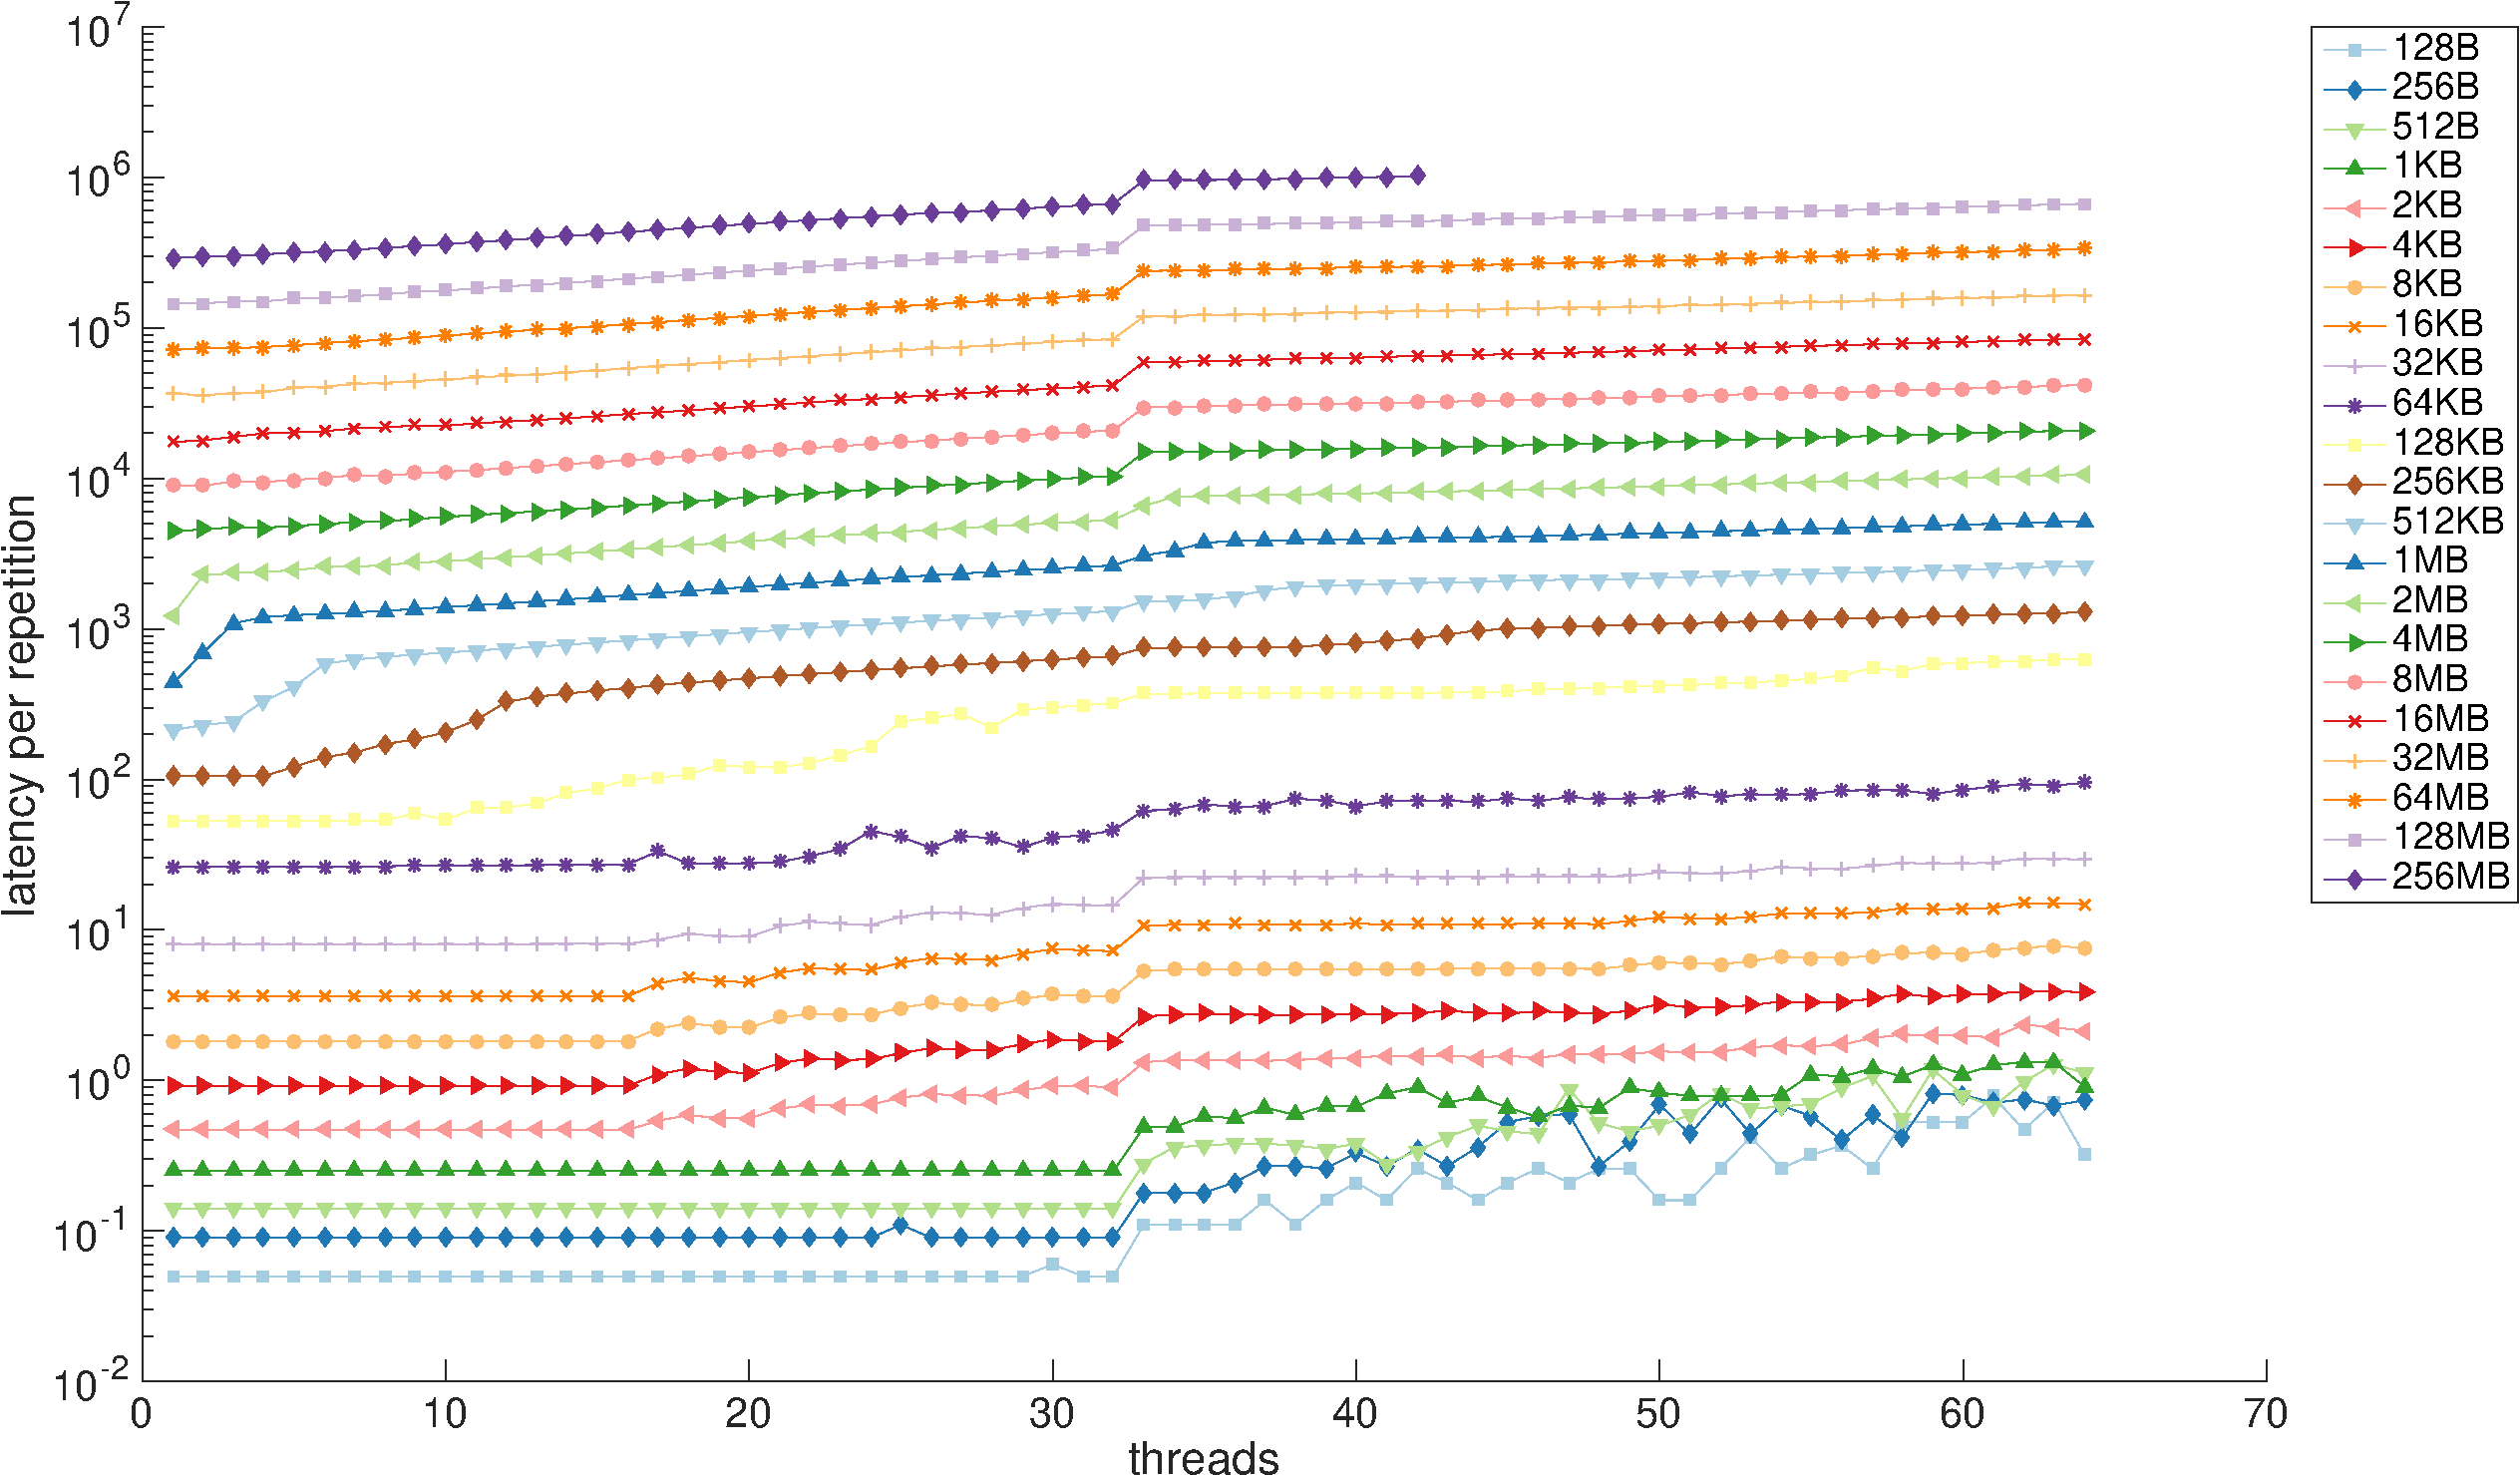
\includegraphics[width=\textwidth]{images/mem-latency.pdf}
    \caption{Memory latency of the CN6880 in microseconds across number of threads for integer data type (32bit), measured by MPAC. Each data point in the graph present one experiment run with different thread and write sizes. The latencies for different packet sizes are marked with colors as shown in the legend (in bytes). The y-axis is presented in logarithmic scale.}
    \label{fig:mem-latency}
  \end{center}
\end{figure}

Figure~\ref{fig:mem-latency} presents the results from the latency measurements for different packet sizes and thread counts. Notice that the y-axis the graph is logarithmic. As expected, the memory latencies grow together with the size of the write. The transition between the memory levels (32K L1, 4MB L2~\cite{cavium:2010:fundamentals}) can be seen as the jumps in the latency graph. With 128B - 1KB write sizes both the read and write arrays fit in the L1 cache (32KB~\cite{cavium:2010:fundamentals}), and thus the latency per repetition is independent of the thread count. With write sizes above 2KB, some of the writes hit L2 cache (4MB~\cite{cavium:2010:fundamentals}), increasing the latency as the thread count increases. Similarly, the step from L2 cache to RAM can be seen 128KB, 256KB, 512KB, 1MB, and 2MB write sizes, where both write and read arrays completely fit in the L2 cache with 8, 4, 2, 1 and 1 threads, and move to RAM beyond that.

The write latencys also thrash beyond 32 threads, especially for the cache sizes. This does not affect the main core memory accesses in the model, as only 32 threads are used for packet processing. However, these numbers work as a reference when modeling the memory communication of other units such as SSO.

\begin{figure}[]
  \begin{center}
    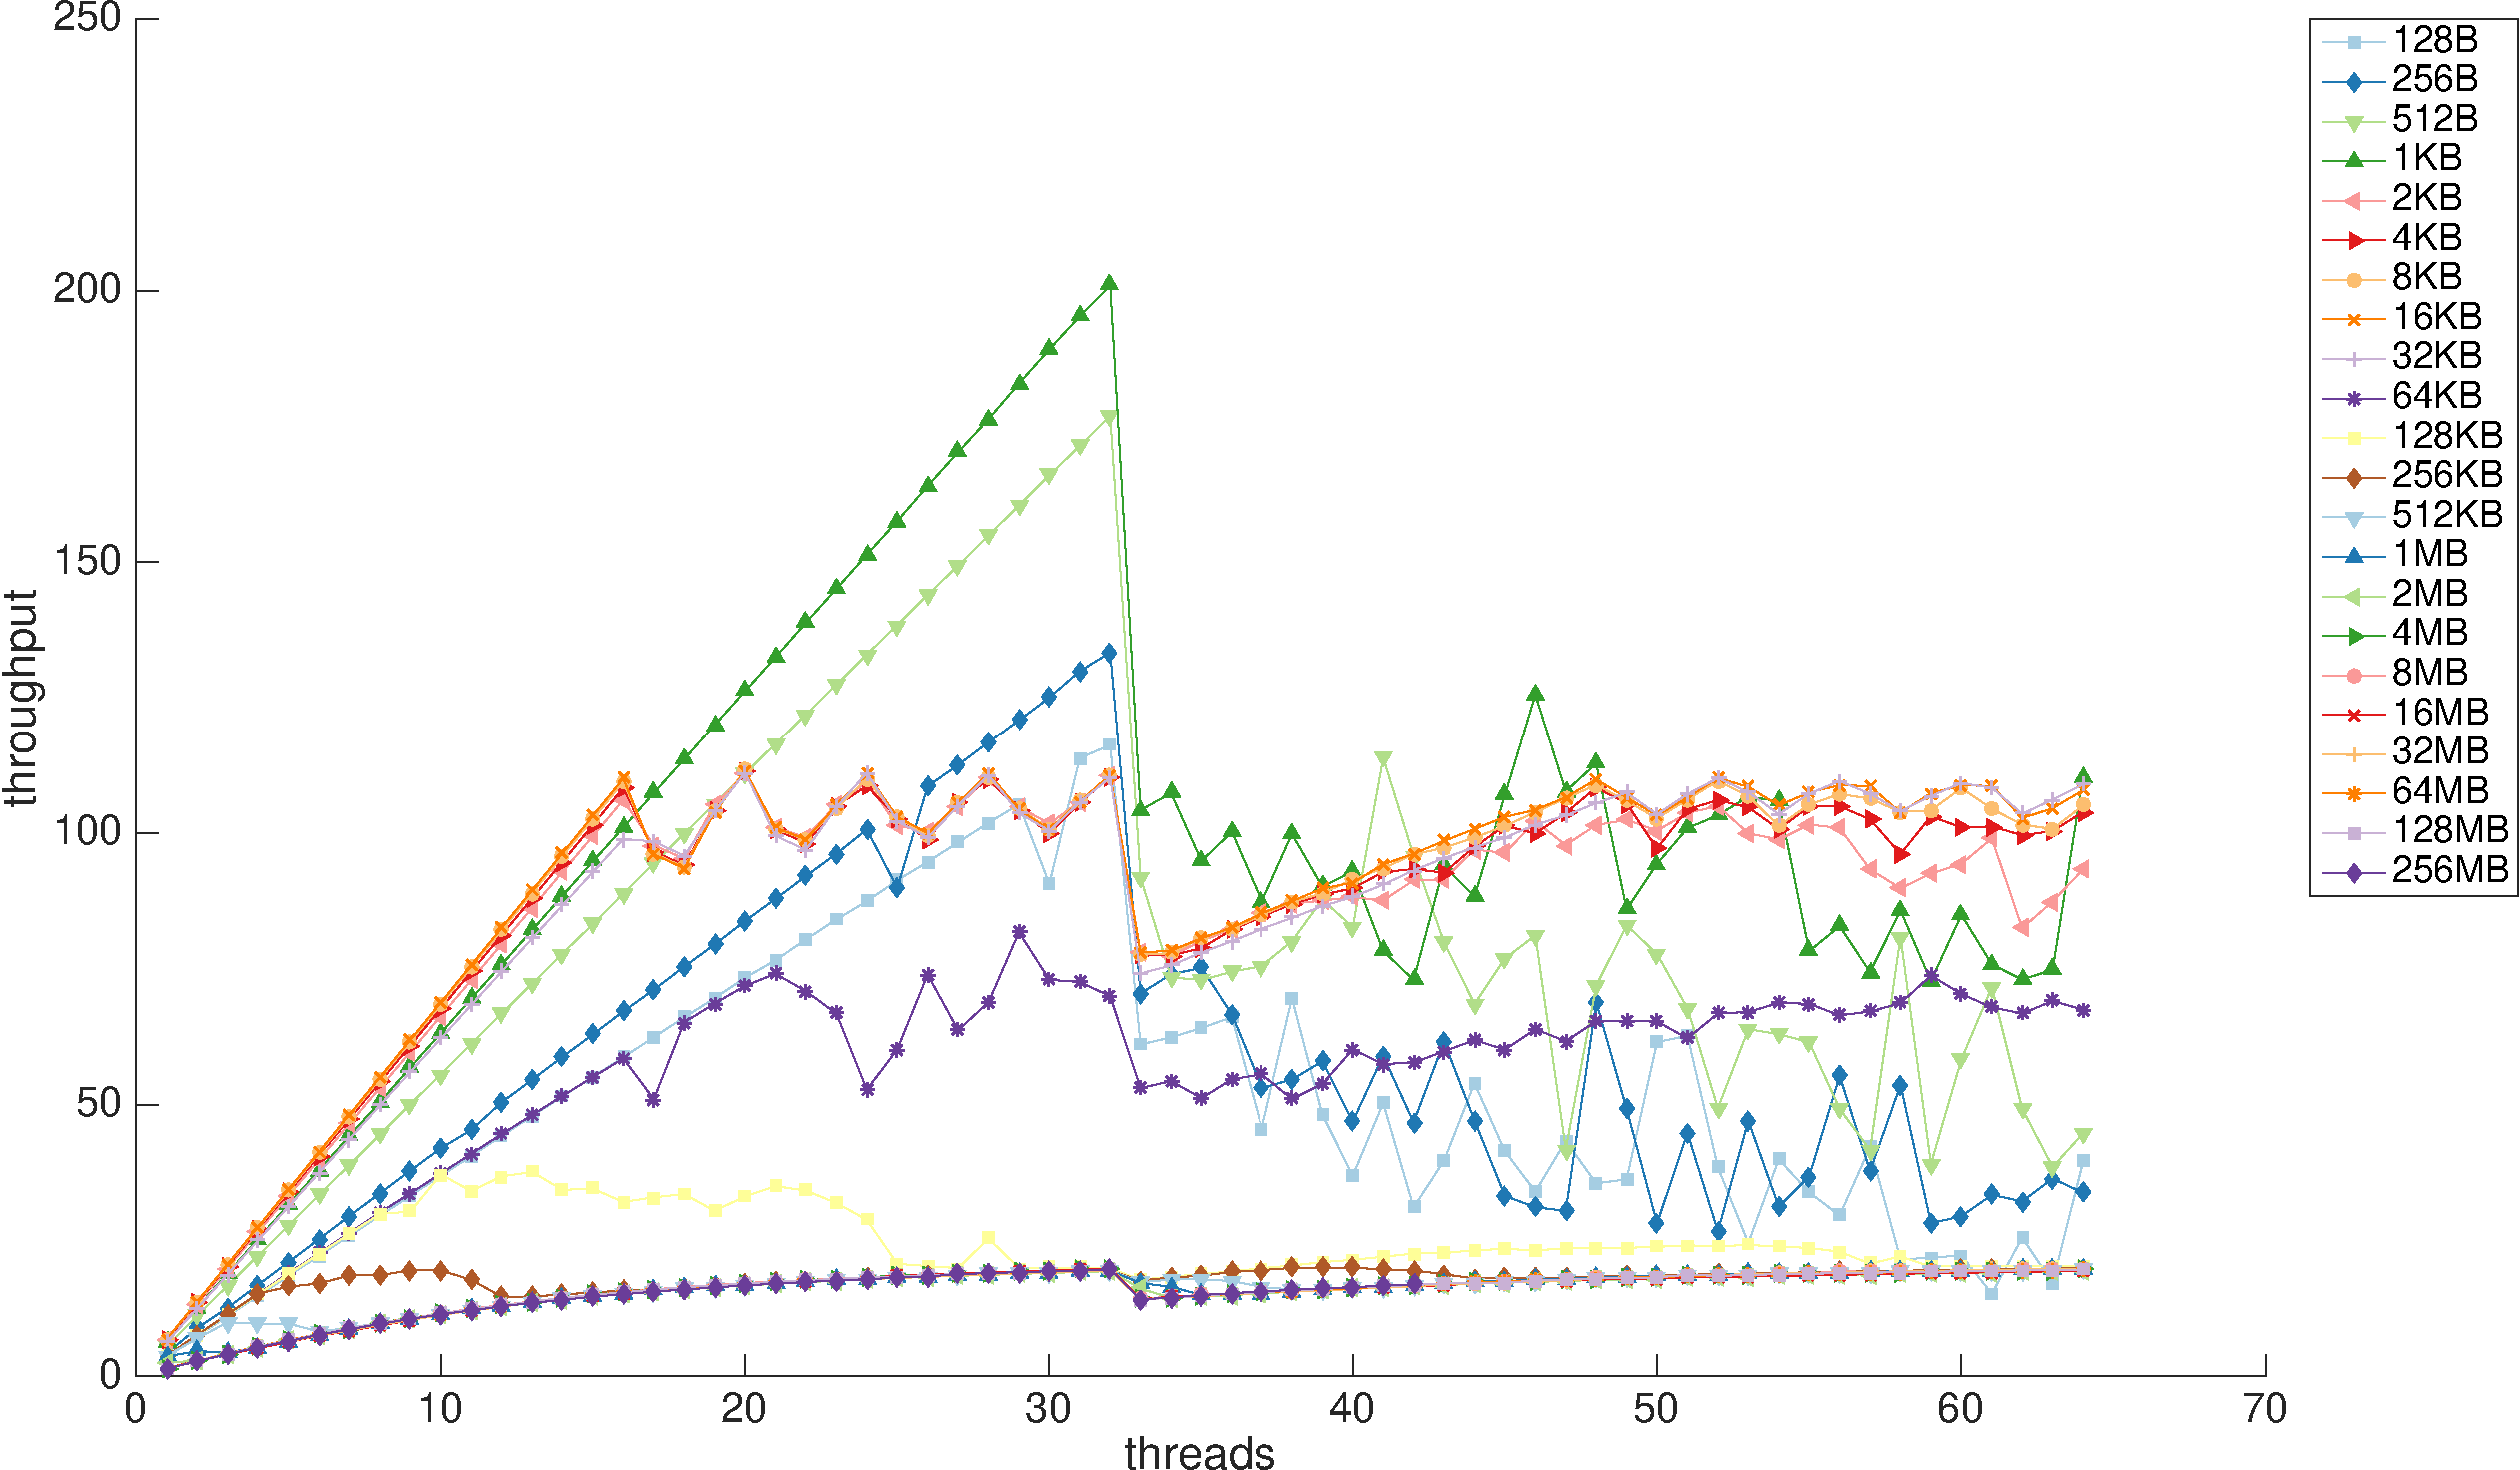
\includegraphics[width=\textwidth]{images/mem-throughput.pdf}
    \caption{Memory throughput of the CN6880 in Gbps across number of threads for integer data type (32bit), measured by MPAC. Each data point in the graph present one experiment run with different thread and data sizes. The throughput for different packet sizes are marked with colors as shown in the legend (in bytes).}
    \label{fig:mem-throughput}
  \end{center}
\end{figure}

Figure~\ref{fig:mem-latency} presents the results from the throughput measurements for different packet sizes and thread counts. Again, as expected, the maximum throughput is achieved with 1KB write lengths and 32 cores, when both the write and read arrays fit in the caches. The write throughput scales linearly with 128B - 1KB write sizes for up to 32 cores, with 2KB - 64KB up to 16 cores, and for 256KB, 512KB, and 1MB, write sizes up to 8, 4, and 2 cores respectively. The transition between the memory levels are similar as in the latency graph. Again, a clear thrashing can be seen with more than 32 threads.

\section{Simulation Model}
\label{sec:simulation-model}

We created a high level simulation model of the Cavium OCTEON II CN6880 network processing unit with Performance Simulation Environment. As our interests are mainly in the applications' and SSO unit's  effect on the packet throughput and latency, we will not model the specific details of all the hardware components. Some of the components, such as the input and output phases, or the memory models, are modeled statistically. Figure~\ref{fig:full-model} shows a layered representation of the main components of the final model: workload, hardware, and software. The workload model and software model's application steps vary between different applications, and are not fixed part of the CN6880 model per se, but rather presented here to give a full example of the model.

\begin{figure}[]
  \begin{center}
    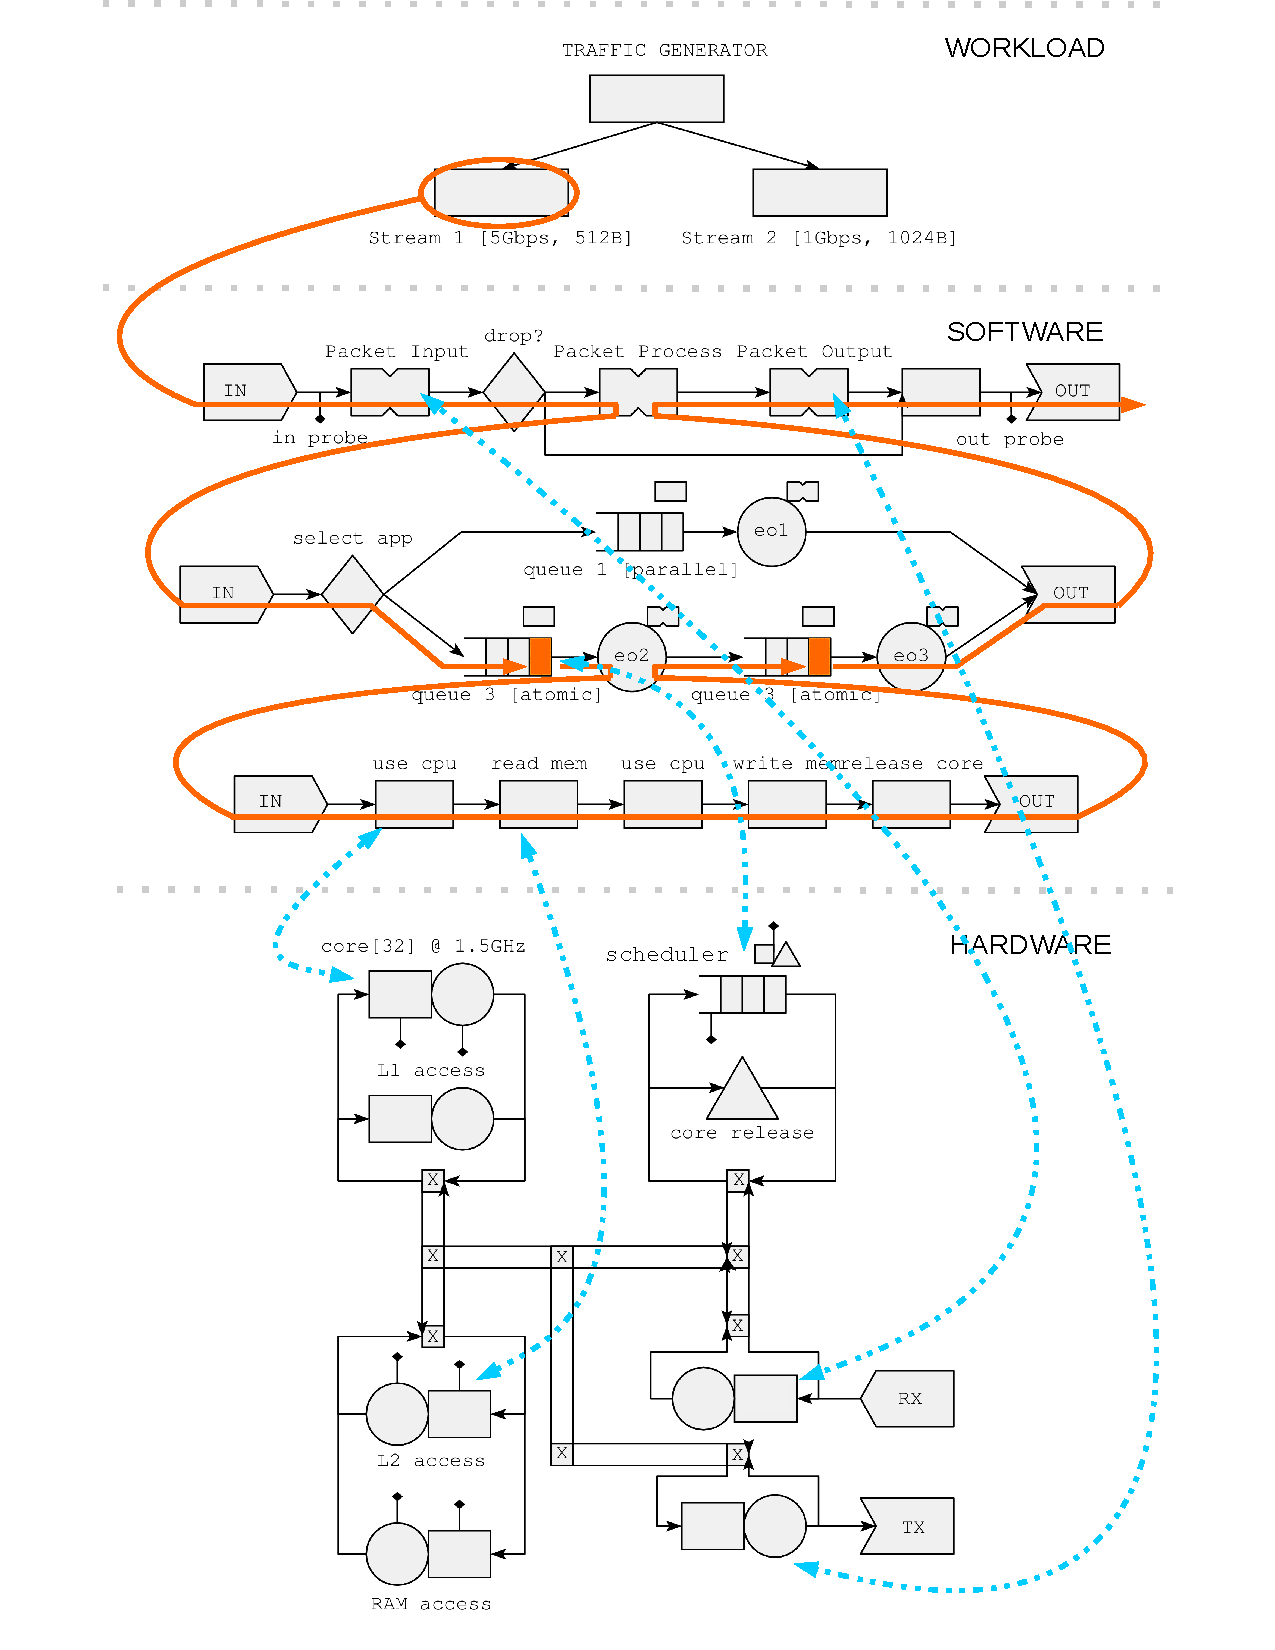
\includegraphics[width=\textwidth]{images/pse-models/fullmodel.pdf}
    \caption{Graphical presentation of the OCTEON II CN6880 PSE model. The workload model (top) generates network packets, which then flow through the software model (middle), consuming the hardware resources (bottom). The orange arrows represent an example of a packet's path through the software model, and the blue arrows the resource usage at each software model node.}
    \label{fig:full-model}
  \end{center}
\end{figure}

The workload model, at the top of the picture, consists of two packet streams. The TRAFFIC GENERATOR node activates the two stream nodes, which again generate packets that enter the software layer. The workload nodes contain parameters, such as the application id's, that are used to control the packet flows in the software model.

% has a lifetime of 0.5 seconds, and it triggers the streams with interval drawn from a uniform distribution with parameters 0.00005 and 0.00015. The streams have lifetime of 0.0004 seconds, and interval drawn from a lognormal distribution. The packet sizes of the streams are defined with the size attribute. Both of the streams also specify an appId attribute that is used to define the processing application in the software model. The packets from both streams enter the IN node of the top level software model.

The software model is divided into several submodels. The top software level model consists of packet input, packet processing and packet output submodels. The submodel view of the packet input and packet output are omitted from the picture for the sake of simplicity, as in both of these phases, the core and memory usage is linearly dependent on the packet size with additional Gaussian noise. In the input phase, the packet consumes specific amount of core cycles for the header processing, and copies the packet header and the packet data to the memory. Packet output node copies the packet from the memory, and consumes certain amount of clock cycles for the packet checksum calculations.

The packet processing submodel is presented in the middle software layer. The select app node forwards each of the packets to one of the two packet processing application, based on the application id attribute defined in the workload model. The queue nodes represent the core scheduling done by the SSO hardware unit. The packets arriving in the upper application have priority of 1, and they can be processed in parallel. In the application below, there are 2 atomic queues with priority 3. When the packet receives the passive resource from SSO, it can enter the actual processing application, called execution object (eo). The execution objects are submodels that consume core cycles and memory similarly to the packet input and packet output submodels presented above. The SSO/core passive resource is released inside each execution object.

The hardware model is a simple one level model containing no submodels. In the bottom left hand corner, there are PKI and PKO devices providing processor cycles for the packet input and packet output phases. The only passive resource node, SSO, provides core access resources, that can be released with the core release node. The application cores are shown in the top left corner of the hardware layer. There are 32 cores, and a specific L1 cache access for each of them. The L2 and RAM memory resources provide the delay for reading and writing to memory.

The probes, attached to the SSO unit, the cores, and the memory nodes, are used to gather statistics from the execution. Each of the units have two probes, one to measure the resource usage, and the other to measures the queue for the corresponding resource. In this hardware model, the routing nodes (squares) and the edges connecting the resources do not have any functional meaning, but are used solely to mimic the graphical models of the CN6880 unit presented in~\cite{cavium:2010:fundamentals}.


%%% Local Variables:
%%% mode: latex
%%% TeX-master: "thesis-hartikainen"
%%% End:
